\documentclass[border=10pt]{standalone}
%%%<
\usepackage{verbatim}
%%%>
\usepackage{pgfplots}
\pgfplotsset{width=7cm,compat=1.8}
\begin{comment}
:Title: Cylindric spiral
:Tags: 3D;Color maps
:Author: Jake
:Slug: cylinder-spiral

We would like to make an image  to illustrate the construction of
a spiral capacitor. These are made of spiral coiled films. It's
like a rectangular paper tailed around one side.

This example was written by Jake on TeX.SE.
\end{comment}
\pgfplotsset{
    colormap/outside/.style={
        colormap=
            {outside}{
            rgb255(0cm)=(110,110,255);
            rgb255(1cm)=(20,20,255);
            }
    },
    colormap/outside,
    colormap/inside/.style={
        colormap={inside}{
            rgb255(0cm)=(20,20,255);
            rgb255(1cm)=(220,220,255);
        }
    },
    colormap/inside
}
\begin{document}
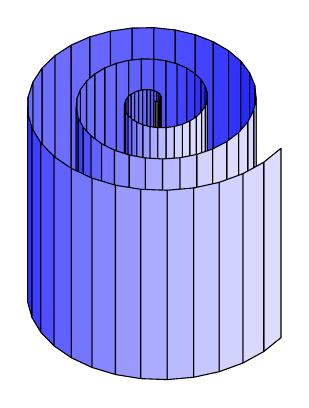
\begin{tikzpicture}
  \begin{axis}[
      hide axis,
      axis equal image,
      z buffer=sort,
      view={30}{40},
      width=15cm
    ]
    \addplot3 [
      surf,
      domain=0:3*360,
      samples=100,
      y domain=0:2000,
      samples y=2,
      line join=round,
      mesh/interior colormap name=inside,
      colormap/outside,
      shader=faceted,
      variable=\t,
      point meta={cos(t)},
      faceted color=black,
    ]
    ( {cos(t)*1.1*t},{sin(t)*1.1*(t)},{y} );
  \end{axis}
\end{tikzpicture}
\end{document}
